\chapter{Introdução}
\label{chap:intro}

\section{Descrição do Problema}
\label{sec:desc}

A diarização de locutor consiste no processo de identificar os diferentes locutores em um conteúdo multimídia de forma a separa-los temporalmente, definindo quando quem falou, e produzir um tipo de roteiro para o mesmo.

Tradicionalmente, tenta-se resolver esse problema através da análise exclusiva do áudio, por meio da extração de \textit{features} na forma de vetores denominados \textit{I-vectors}\cite{zewoudieUseLongtermFeatures2018}, e subsequente clusterização destes.
Porém, trata-se de um problema difícil; o timbre, principal característica sonora responsável pela identificação do locutor pelo ser humano, é de caráter neurológico \cite{oxenhamPitchPerception2012}, produzido pela decomposição da onda sonora em seus harmônicos pelo trato auditivo.
E, ainda, como propriedade intrínseca da etapa de clusterização, a utilização desses algoritmos depende do conhecimento prévio do número de locutores que participam do áudio.

Dadas essas limitações, temos que o desempenho dos algoritmos considerados estado da arte é insuficiente, com taxa de erro de diarização (a partir daqui chamada de DER, do inglês \textit{Diarization Error Rate}) de cerca de 20\% nas bases tradicionais.
Portanto, a busca de outras técnicas capazes de prover um melhor desempenho nos leva a considerar também outros sinais constituintes do conteúdo multimídia, como o de vídeo do orador.

\section{Motivação}
\label{sec:motiv}

Em muitas situações, no processo de transcrição de áudio e vídeo, é interessante obter também a informação de quem está falando.
Com essa informação seria possível roteirizar a mídia, viabilizando um melhor entendimento e formatação do texto transcrito.
Além disso, essa informação adicional permite viabilizar novos critérios de busca sobre o texto transcrito, tornando possível filtrar os resultados por locutor.

\section{Definição do Problema}
\label{sec:problem-desc}

O problema de diarização de locutor consiste em particionar automaticamente um sinal de áudio tal que cada uma das partições geradas contenha as falas de um único locutor.
Trata-se de um problema muito relevante à área de reconhecimento de voz, já que entender quem falou em cada momento de uma gravação nos permite contextualizar diversos tópicos que dependem desse tipo de informação para sua legibilidade e interpretação, tais como a geração automática de transcrições de depoimentos judiciais e relatórios médicos eletrônicos.

A solução proposta neste trabalho consiste em construir um sistema capaz de diarizar as falas de um único locutor em tempo real a partir de um vídeo frontal do mesmo, intuição da qual se encontra demonstrada na figura \ref{fig:intuition}.
Para isso, o sistema de diarização deve ser capaz de, a partir de uma sequência de quadros extraída do vídeo original, determinar se o objeto da gravação está ou não falando.
Neste trabalho iremos desconsiderar o áudio associado, já que o processamento deste foge à área de visão computacional.

\begin{figure}[h]
    \centering
    \resizebox{\textwidth}{!}{
        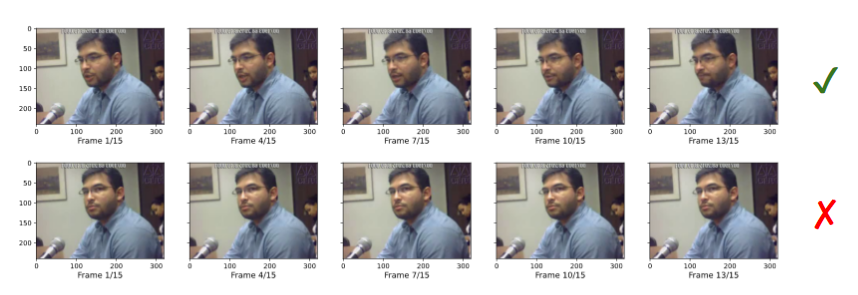
\includegraphics{figures/intro_intuition.png}
    }
    \caption{Intuição por trás desta proposta de solução. Note a facilidade de se identificar corretamente a fala do locutor mesmo quando apresentados apenas poucos quadros de um segmento contínuo.}
    \label{fig:intuition}
\end{figure}

Com esta finalidade, propomos uma arquitetura em três etapas:
\begin{enumerate}
    \item Com o uso de um identificador facial, o sistema identificará rostos nas imagens que lhe forem fornecidas. 
    \item Pontos de referência relevantes serão extraídos dos rostos identificados. 
    \item Através de um modelo de aprendizado de máquina previamente treinado, o sistema deverá ser capaz de determinar se o sujeito identificado está ou não falando.
\end{enumerate}

\section{Escopo}
\label{sec:scope}

De forma geral, gostaríamos de identificar as falas de todos os oradores do texto.
No entanto, muitas vezes é suficiente identificar apenas um destes, por exemplo no caso de audiências e depoimentos do Tribunal de Justiça.
Nesse caso específico desejamos identificar com maior precisão os trechos falados pelo depoente, independentemente do número de participantes da audiência, de forma a distinguir futuramente o que foi dito pelo mesmo em seu depoimento.

Para esta finalidade, assumimos que esteja disponível um vídeo frontal da face do locutor (depoente), além do áudio combinado de todos os participantes, em canal monoaural.
Esta suposição é feita tendo em vista as características dos dados reais, tendo o conhecimento de que caso o áudio estivesse separado em canais correspondentes a cada locutor o problema se tornaria trivial.
Assim, este trabalho ficará limitado a tratar de casos nos quais estas informações estejam disponíveis, e com a determinação de que o vídeo deve ser de boa qualidade.

\section{Estrutura do Trabalho}
\label{sec:structure}

Este trabalho se encontra organizado da seguinte maneira:

No capítulo 2 apresentamos a fundamentação teórica referente às técnicas e tecnologias utilizadas na implementação de cada uma das etapas propostas nesse trabalho.
Em um primeiro momento, fazemos uma revisão das abordagens e implementações formuladas para resolução do problema de alinhamento facial até hoje. 
Em seguida, apresentamos os conceitos e técnicas críticas para nossa implementação, sendo estas as redes neurais convolucionais, detecção de objetos por histograma de gradientes orientados, e alinhamento facial.

No capítulo 3 apresentamos a nossa implementação do sistema proposto. 
Abordamos tópicos como as ferramentas utilizadas, pré-processamento dos dados de treinamento, e a arquitetura proposta para a rede neural convolucional.
Por fim, discutimos a implementação da aplicação final, para lidar com dados não tratados previamente.

No capítulo 4 demonstramos os resultados de nosso método quando aplicado sobre dataset fornecido pela Defensoria Pública do Estado do Rio de Janeiro, que contém vídeos dos participantes individuais com as características desejadas.

Por fim, no capítulo 5, resumimos e apresentamos nossas conclusões quanto ao trabalho realizado, discutindo os resultados obtidos e os fatores que contribuíram para estes, e enumeramos trabalhos futuros a serem realizados sobre o mesmo tema.

\section{Código Fonte}
\label{sec:source-code}

Todo o código fonte desenvolvido para este trabalho pode ser obtido online no repositório do GitHub em \url{https://github.com/RenanBasilio/SpeechActionClassifier}.